% Compilation : pdflatex B2.tex (deux fois).
% Document autonome : texte, formules et figures TikZ modifiables.
% Les reperes Source renvoient aux pages du manuscrit.
\documentclass[11pt,a4paper]{article}
\usepackage[utf8]{inputenc}
\usepackage[T1]{fontenc}
\usepackage[provide=*,french]{babel}
\usepackage[scaled=.95]{helvet}
\renewcommand{\familydefault}{\sfdefault}
\usepackage{amsmath,amssymb,esint,array,tabularx}
\usepackage{geometry}
\geometry{left=15mm,right=15mm,top=18mm,bottom=18mm,headheight=14pt,headsep=6mm}
\usepackage{fancyhdr,lastpage,tikz}
\usetikzlibrary{arrows.meta,calc,decorations.pathreplacing,decorations.pathmorphing,decorations.markings,patterns}
\usepackage[most]{tcolorbox}
\usepackage{enumitem,titlesec,needspace,hyperref}
\hypersetup{hidelinks,pdftitle={Équations de Maxwell : généralités},pdfsubject={Cours de physique}}
\pagestyle{fancy}\fancyhf{}
\fancyhead[L]{\footnotesize Physique B2 - Équations de Maxwell : Généralités - inspiré par les cours de Mme Mesnil}
\fancyhead[R]{\small\thepage/\pageref{LastPage}}
\fancyfoot[R]{\small PC-PC*}
\renewcommand{\headrulewidth}{0pt}
\clubpenalty=10000\widowpenalty=10000\displaywidowpenalty=10000
\setlength{\parindent}{0pt}\setlength{\parskip}{4pt}
\setlength{\abovedisplayskip}{6pt}\setlength{\belowdisplayskip}{6pt}
\AtBeginEnvironment{center}{\setlength{\topsep}{4pt}\setlength{\partopsep}{0pt}}
\setlist[itemize]{leftmargin=5mm,itemsep=3pt,topsep=3pt,label=\(\rightarrow\)}
\setlist[enumerate]{leftmargin=6mm,itemsep=3pt,topsep=3pt}
\renewcommand{\thesection}{\Roman{section}}
\renewcommand{\thesubsection}{\thesection.\arabic{subsection}}
\titleformat{\section}{\Large\bfseries}{\thesection.}{.4em}{}
\titleformat{\subsection}{\large\bfseries}{\thesubsection.}{.4em}{}[\titlerule]
\titleformat{\subsubsection}{\normalsize\bfseries}{\alph{subsubsection})}{.5em}{}
\titlespacing*{\section}{0pt}{11pt}{6pt}
\titlespacing*{\subsection}{0pt}{9pt}{5pt}
\titlespacing*{\subsubsection}{0pt}{8pt}{4pt}
\newtcolorbox{cadre}[1][]{enhanced,sharp corners,colback=white,colframe=black,boxrule=1.1pt,left=7pt,right=7pt,top=5pt,bottom=5pt,before skip=7pt,after skip=7pt,#1}
\newtcolorbox{exemple}[1][]{enhanced,breakable,sharp corners,colback=white,colframe=black,boxrule=.7pt,left=8pt,right=8pt,top=6pt,bottom=6pt,before skip=8pt,after skip=8pt,#1}
\tcbset{etoiles/.style={width=\dimexpr\linewidth-22mm\relax,overlay={\node[anchor=west,inner sep=0pt,font=\small] at ([xshift=2mm]frame.east) {\(#1\)};}}}
\newcommand{\zone}[1]{\tikz[baseline=(z.base)]\node[draw,circle,inner sep=1pt,font=\scriptsize,minimum size=3.5mm](z){#1};}
\newcommand{\dd}{\mathrm d}
\newcommand{\vv}{\vec v}
\newcommand{\grad}{\overrightarrow{\mathrm{grad}}}
\newcommand{\pd}[2]{\frac{\partial #1}{\partial #2}}
\newcommand{\ux}{\vec u_x}\newcommand{\uy}{\vec u_y}\newcommand{\uz}{\vec u_z}
\newcommand{\cste}{\mathrm{cste}}
\newcommand{\titr}[1]{\par\Needspace{4\baselineskip}\textbf{\underline{#1}}\par\nopagebreak[3]}
\newcommand{\planpart}[2]{\par\vspace{5pt}{\bfseries #1. #2}\par}
\newcommand{\plansub}[2]{\hspace*{7mm}{\itshape #1) #2}\par}
\newcommand{\plansubsub}[1]{\hspace*{15mm}{\itshape #1}\par}
\tikzset{>=Stealth,every node/.style={font=\small},flow/.style={thick,->},edge/.style={thick}}
\newcommand{\stars}[1]{\mathord{\star}\ifnum#1>1\mkern5mu\mathord{\star}\fi\ifnum#1>2\mkern5mu\mathord{\star}\fi\ifnum#1>3\mkern5mu\mathord{\star}\fi\ifnum#1>4\mkern5mu\mathord{\star}\fi\ifnum#1>5\mkern5mu\mathord{\star}\fi}
\newenvironment{result}[1][4]{\begin{cadre}[etoiles={\stars{#1}}]}{\end{cadre}}
\newcommand{\vj}{\vec j}\newcommand{\vE}{\vec E}\newcommand{\vB}{\vec B}
\newcommand{\vPi}{\vec\Pi}\newcommand{\rot}{\overrightarrow{\mathrm{rot}}}
\newcommand{\divg}{\operatorname{div}}\newcommand{\sy}{\operatorname{sym}}
\newcommand{\D}{\mathcal D}\newcommand{\R}{\mathcal R}
\newcommand{\fig}[1]{\begin{center}#1\end{center}}
\definecolor{charge}{RGB}{155,50,165}
\definecolor{current}{RGB}{195,40,45}
\tikzset{arr/.style={thick,->},cur/.style={current,thick,->},el/.style={charge,thick,->},mag/.style={green!50!black,thick,->},pt/.style={circle,fill,inner sep=1.2pt},plane/.style={blue!55!black,thin}}
% Figures entièrement modifiables en TikZ.
\newcommand{\slicecharge}{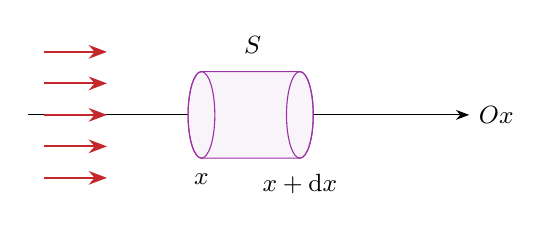
\begin{tikzpicture}
\draw[->](-2.2,0)--(3.4,0)node[right]{$Ox$};
\draw[charge,fill=charge!6](0,-.55)--(1.25,-.55)arc(-90:90:.17 and .55)--(0,.55)arc(90:270:.17 and .55);
\draw[charge](0,0)ellipse(.17 and .55)(1.25,0)ellipse(.17 and .55);
\node[below]at(0,-.63){$x$};\node[below]at(1.25,-.63){$x+\dd x$};\node[above]at(.65,.65){$S$};
\foreach\y in{-.8,-.4,0,.4,.8}{\draw[cur](-2,\y)--(-1.2,\y);}
\end{tikzpicture}}
\newcommand{\closedvolume}{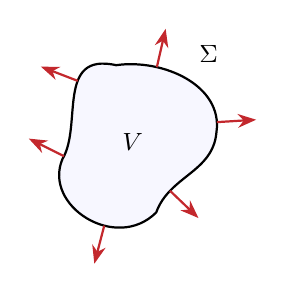
\begin{tikzpicture}[scale=.85]
\draw[thick,fill=blue!3,postaction={decorate},decoration={markings,mark=at position .08 with {\draw[cur](0,0)--(0,.5);},mark=at position .25 with {\draw[cur](0,0)--(0,.5);},mark=at position .42 with {\draw[cur](0,0)--(0,.5);},mark=at position .58 with {\draw[cur](0,0)--(0,.5);},mark=at position .76 with {\draw[cur](0,0)--(0,.5);},mark=at position .91 with {\draw[cur](0,0)--(0,.5);}}]
(0,1.2)..controls(.7,1.3)and(1.6,.9)..(1.5,.2)..controls(1.45,-.4)and(.8,-.45)..(.6,-1)..controls(0,-1.6)and(-1.1,-.9)..(-.8,-.2)..controls(-.5,.3)and(-.9,1.4)..(0,1.2);
\node at(.25,.05){$V$};\node[above right]at(1.1,1.1){$\Sigma$};
\end{tikzpicture}}
\newcommand{\chargesplit}{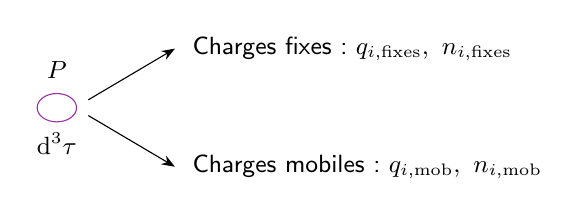
\begin{tikzpicture}
\draw[charge](0,0)ellipse(.25 and .18);\node[above]at(0,.25){$P$};\node[below]at(0,-.2){$\dd^3\tau$};
\draw[->](.4,.1)--(1.5,.75);\draw[->](.4,-.1)--(1.5,-.75);
\node[right,align=left]at(1.6,.75){Charges fixes : $q_{i,\mathrm{fixes}},\ n_{i,\mathrm{fixes}}$};
\node[right,align=left]at(1.6,-.75){Charges mobiles : $q_{i,\mathrm{mob}},\ n_{i,\mathrm{mob}}$};
\end{tikzpicture}}
\newcommand{\copper}{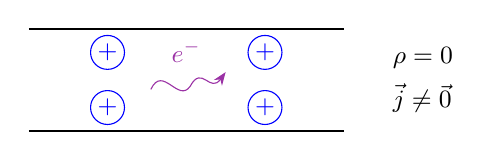
\begin{tikzpicture}
\draw[thick](-2,.65)--(2,.65)(-2,-.65)--(2,-.65);
\foreach\x in{-1,1}{\foreach\y in{-.35,.35}{\node[draw,circle,blue,inner sep=1pt]at(\x,\y){$+$};}}
\draw[charge,->](-.45,-.12)..controls(-.3,.2)and(-.1,-.3)..(.05,-.08)..controls(.2,.2)and(.3,-.18)..(.5,.1);\node[charge,above]at(0,.1){$e^-$};
\node[right,align=left]at(2.5,0){$\rho=0$\\[5pt]$\vj\ne\vec0$};
\end{tikzpicture}}
% Distribution symétrique (#1=0) ou antisymétrique (#1=1).
\newcommand{\distribsym}[1]{\begin{tikzpicture}[scale=.85]
\fill[blue!5](-1.6,0)..controls(-1.7,1)and(-.6,1.4)..(0,.85)..controls(.6,1.4)and(1.7,1)..(1.6,0)..controls(1.5,-1)and(.5,-1.3)..(0,-.75)..controls(-.5,-1.3)and(-1.5,-1)..cycle;
\draw[blue!60!black,thick](-1.6,0)..controls(-1.7,1)and(-.6,1.4)..(0,.85)..controls(.6,1.4)and(1.7,1)..(1.6,0)..controls(1.5,-1)and(.5,-1.3)..(0,-.75)..controls(-.5,-1.3)and(-1.5,-1)..cycle;
\draw(0,-1.5)--(0,1.6)node[above]{$\Pi$};\draw[dashed](-.8,0)--(.8,0);
\node[pt]at(-.8,0){};\node[below]at(-.8,0){$P$};\node[pt]at(.8,0){};\node[below]at(.8,0){$P'$};
\draw[cur](-.8,0)--(-1.3,.8)node[above left]{$\vj(P,t)$};
\node[below]at(-1,-1.05){$\rho(P,t)$};
\ifnum#1=0
\draw[cur](.8,0)--(1.3,.8)node[above right]{$\vj(P',t)$};\node[below]at(1,-1.05){$\rho(P',t)$};
\else
\draw[current,dashed,->](.8,0)--(1.3,.8);\node[right,align=left,current]at(1.5,.9){$\sy_\Pi[\vj(P,t)]$};
\draw[cur](.8,0)--(.3,-.8);\node[right,current]at(.75,-1.3){$\vj(P',t)$};\node[right]at(1.7,-.25){$\rho(P',t)=-\rho(P,t)$};
\fi\end{tikzpicture}}
\newcommand{\lorentzsym}{\begin{tikzpicture}
\draw(0,-1)--(0,1.8)node[above]{$\Pi$};\draw[dotted](-1.7,0)--(1.7,0);
\foreach\s in{-1,1}{\node[pt]at(\s*1.7,0){};\node[above]at(\s*1.7,.05){$q$};\draw[cur](\s*1.7,0)--(\s*2.05,1)node[above]{$\vv_\R$};\draw[el](\s*1.7,0)--(\s*2.9,.55);}
\node[below]at(-1.7,0){$P$};\node[below]at(1.7,0){$P'$};\node[charge,left]at(-2.9,.55){$\vec F_P$};\node[charge,right]at(2.9,.55){$\vec F_{P'}$};
\end{tikzpicture}}
% Deux illustrations du caractère axial de B.
\newcommand{\axialfield}[1]{\begin{tikzpicture}
\draw(0,-.95)--(0,1.7)node[above]{$\Pi$};
\foreach\s in{-1,1}{\node[pt]at(\s*1.75,0){};\draw[cur](\s*1.75,0)--(\s*1.25,.7);\node[current]at(\s*1.1,.9){$\vv$};\node[below]at(\s*1.75,-.15){$q>0$};}
\ifnum#1=0
\draw[el](-1.75,0)--(-2.55,1);\draw[el](1.75,0)--(2.55,1);
\node[charge,above]at(-2.55,1){$\vec F$};\node[charge,above]at(2.55,1){$\vec F$};
\node[green!50!black,left]at(-2.1,-.05){$\vB\ \otimes$};\node[green!50!black,right]at(2.1,-.05){$\vB\ \odot$};
\else
\draw[mag](-1.75,0)--(-2.8,0)node[below]{$\vB$};\draw[mag](1.75,0)--(.7,0)node[below]{$\vB$};
\node[charge]at(-1.75,0){$\bigodot$};\node[charge,right]at(-1.65,.2){$\vec F$};\node[charge]at(1.75,0){$\bigodot$};\node[charge,right]at(1.85,.2){$\vec F$};
\fi\end{tikzpicture}}
% Composantes parallèles et perpendiculaires dans un plan de symétrie (0) ou d'antisymétrie (1).
\newcommand{\components}[1]{\begin{tikzpicture}[scale=.95]
\draw(0,-1.65)--(0,1.9)node[above]{$\ifnum#1=0\Pi\else\Pi'\fi$};
\node[pt]at(-2.7,0){};\node[below]at(-2.7,-.15){$M$};
\draw[cur](-2.7,0)--(-2.7,1.1);\draw[cur](-2.7,0)--(-3.8,0);\draw[cur](-2.7,0)--(-3.8,1.1);\draw[current,dotted](-3.8,0)--(-3.8,1.1)--(-2.7,1.1);
\node[current,above left]at(-3.8,1.15){$\vE(M,t)$};\node[current,left]at(-3.8,-.15){$\vE_\perp(M,t)$};\node[current,above]at(-2.5,1.2){$\vE_\parallel(M,t)$};
\node[pt]at(2.7,0){};
\ifnum#1=0
\draw[cur](2.7,0)--(2.7,1.1);\draw[cur](2.7,0)--(3.8,0);\draw[cur](2.7,0)--(3.8,1.1);\draw[current,dotted](2.7,1.1)--(3.8,1.1)--(3.8,0);
\node[current,above right]at(3.8,1.15){$\vE(M',t)$};\node[current,right]at(3.8,-.15){$\vE_\perp(M',t)$};\node[current,above]at(2.5,1.2){$\vE_\parallel(M',t)$};
\node[below]at(2.7,-.35){$M'=\sy_\Pi(M)$};
\draw[cur](0,.15)--(0,1.05);\node[current,right]at(.1,.45){$\vE$};
\else
\draw[cur](2.7,0)--(2.7,-1.1);\draw[cur](2.7,0)--(1.6,0);\draw[cur](2.7,0)--(1.6,-1.1);\draw[current,dotted](1.6,0)--(1.6,-1.1)--(2.7,-1.1);
\node[current,below right]at(2.8,-1.15){$\vE_\parallel(M',t)$};\node[current,above]at(1.7,.2){$\vE_\perp(M',t)$};\node[current,below left]at(1.5,-1.15){$\vE(M',t)$};
\node[right]at(2.95,.1){$M'=\sy_{\Pi'}(M)$};
\draw[cur](0,.5)--(-.8,.5);\node[current,below]at(-.65,.4){$\vE$};\draw(-.15,.5)--(-.15,.65)--(0,.65);
\fi\end{tikzpicture}}
\newcommand{\energycharge}{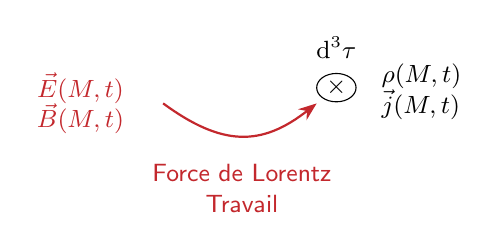
\begin{tikzpicture}
\node[align=center,current]at(-2.3,.25){$\vE(M,t)$\\$\vB(M,t)$};\draw[cur](-1.25,.25)..controls(-.5,-.3)and(0,-.3)..(.7,.25);
\node[current,below,align=center]at(-.25,-.4){Force de Lorentz\\Travail};
\draw(.95,.45)ellipse(.25 and .18);\node at(.95,.45){$\times$};\node[above]at(.95,.7){$\dd^3\tau$};\node[right,align=left]at(1.4,.4){$\rho(M,t)$\\$\vj(M,t)$};
\end{tikzpicture}}
\newcommand{\poyntingsurface}{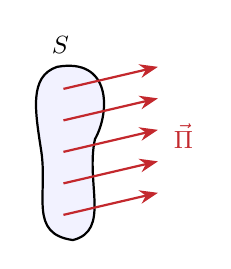
\begin{tikzpicture}[scale=.8]
\draw[thick,fill=blue!5](-.35,1.35)..controls(.5,1.5)and(.5,.65)..(.25,.2)..controls(.1,-.5)and(.5,-1.25)..(-.1,-1.4)..controls(-.8,-1.3)and(-.5,-.7)..(-.6,0)..controls(-.7,.65)and(-.8,1.2)..(-.35,1.35);
\node[above]at(-.3,1.4){$S$};\foreach\y in{-1,-.5,0,.5,1}{\draw[cur](-.25,\y)--(1.25,\y+.35);}\node[current,right]at(1.35,.25){$\vPi$};\end{tikzpicture}}
\newcommand{\stationwire}{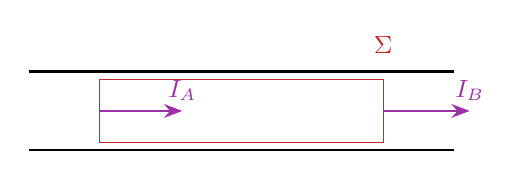
\begin{tikzpicture}
\draw[thick](-2.7,-.5)--(2.7,-.5)(-2.7,.5)--(2.7,.5);
\draw[current](-1.8,-.4)rectangle(1.8,.4);\node[current,above]at(1.8,.6){$\Sigma$};
\draw[el](-1.8,0)--(-.75,0)node[above]{$I_A$};\draw[el](1.8,0)--(2.9,0)node[above]{$I_B$};\end{tikzpicture}}
\newcommand{\junction}{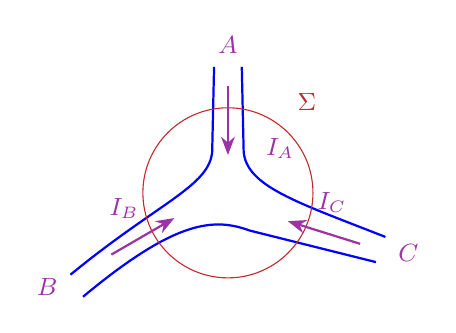
\begin{tikzpicture}[scale=.8]
\draw[blue,thick](-.22,2)--(-.25,.65)..controls(-.3,.1)and(-1.1,-.15)..(-2.5,-1.3);
\draw[blue,thick](.22,2)--(.25,.65)..controls(.3,.1)and(1.1,-.15)..(2.5,-.7);
\draw[blue,thick](-2.3,-1.65)..controls(-.8,-.4)and(-.2,-.4)..(.35,-.6)--(2.35,-1.1);
\draw[current](0,0)circle(1.35);\node[current,above right]at(.95,1.15){$\Sigma$};
\draw[el](0,1.7)--(0,.6);\node[charge,right]at(.45,.7){$I_A$};
\draw[el](-1.85,-.98)--(-.85,-.4);\node[charge]at(-1.65,-.25){$I_B$};
\draw[el](2.1,-.81)--(.95,-.45);\node[charge]at(1.65,-.15){$I_C$};
\node[charge,above]at(0,2.05){$A$};\node[charge,left]at(-2.55,-1.5){$B$};\node[charge,right]at(2.55,-.95){$C$};\end{tikzpicture}}

\begin{document}
{\raggedright\fontsize{27}{31}\selectfont\bfseries Équations de Maxwell : généralités\par}
\vspace{4mm}
\planpart{I}{Postulats de l'électromagnétisme}
\plansub{1}{Conservation de la charge}
\plansubsub{a) Bilan de charges en une dimension}
\plansubsub{b) Bilan de charge : cas général}
\plansub{2}{Force de Lorentz}
\plansub{3}{Équations de Maxwell}
\planpart{II}{Propriétés de symétrie}
\plansub{1}{Propriétés de symétrie d'une distribution}
\plansub{2}{Propriétés de symétrie des champs}
\plansub{3}{Champs en un point d'un plan de symétrie ou d'antisymétrie}
\plansub{4}{Retour sur les équations de Maxwell}
\planpart{III}{Énergie électromagnétique}
\plansub{1}{Puissance fournie par un champ électromagnétique aux porteurs de charges}
\plansub{2}{Équation locale de Poynting}
\plansub{3}{Bilan d'énergie électromagnétique}
\planpart{IV}{Régime stationnaire}
\plansub{1}{Définition}
\plansub{2}{Loi locale de conservation de la charge}
\plansub{3}{Équations de Maxwell : le découplage}
\vspace{3mm}
% Source 1
\textbf{Approche historique :} l'électrostatique, la magnétostatique et l'induction ont été décrites séparément, puis réunies avec les équations de Maxwell.

\textbf{Approche du cours :} on admet les équations de Maxwell pour déduire toutes les lois de l'électromagnétisme.
\section{Postulats de l'électromagnétisme}
\subsection{Conservation de la charge}
\begin{cadre}
Dans un système électriquement isolé, la charge est constante.
\end{cadre}
\begin{itemize}
\item Un système électriquement isolé n'échange pas de charge avec l'extérieur (pas de pile, etc.).
% Source 2
\item Par contraposition, si la charge d'un système varie, il y a un échange de charge avec l'extérieur.
\end{itemize}
\subsubsection{Bilan de charges en une dimension}
\fig{\slicecharge}
Les densités suivantes résultent des charges fixes et mobiles :
\[
\left\{\begin{aligned}
\rho(M,t)&=\rho(x,t),\\
\vj(M,t)&=j(x,t)\ux.
\end{aligned}\right.
\]
On effectue un bilan sur une tranche de surface $S$, comprise entre $x$ et $x+\dd x$, entre $t$ et $t+\dd t$.

\textbf{Système :} il est ouvert, fixe et indéformable.
\[
\dd Q=\rho(x,t)S\dd x.
\]
% Source 3
\[
\frac{\dd Q}{\dd t}=\pd{\rho(x,t)}{t}S\dd x,
\qquad
\frac{\dd Q}{\dd t}=j(x,t)S-j(x+\dd x,t)S.
\]
D'où
\begin{align*}
\pd{\rho(x,t)}{t}S\dd x\dd t
 &=j(x,t)S\dd t-j(x+\dd x,t)S\dd t\\
 &=S\dd t\bigl(j(x,t)-j(x+\dd x,t)\bigr),\\
\pd{\rho}{t}S\dd x\dd t
 &=S\dd t\left(-\pd{j}{x}\right)\dd x.
\end{align*}
\begin{result}[3]
\[\pd{\rho}{t}+\pd{j}{x}=0.\]
\end{result}
\subsubsection{Bilan de charge : cas général}
On considère $\rho(M,t)$ et $\vj(M,t)$.
\begin{center}
\begin{minipage}{.35\linewidth}\centering\closedvolume\end{minipage}\hfill
\begin{minipage}{.58\linewidth}
$\Sigma$ est une surface fermée, fixe et indéformable.

Le bilan de charges entre $t$ et $t+\dd t$ porte sur le système ouvert délimité par $\Sigma$.
\end{minipage}
\end{center}
% Source 4
\[
Q(t)=\iiint_V\rho(P,t)\dd^3\tau,
\qquad
\dd Q=\underbrace{\iiint_V\pd{\rho}{t}\dd^3\tau}_{\text{$\Sigma$ fixe et indéformable}}\dd t.
\]
Or, on a aussi
\[
\dd Q=-\oiint_\Sigma\vj\cdot\dd\vec S\,\dd t.
\]
D'où
\[
\iiint_V\pd{\rho}{t}\dd^3\tau=-\oiint_\Sigma\vj\cdot\dd\vec S,
\qquad
\iiint_V\pd{\rho}{t}\dd^3\tau+\oiint_\Sigma\vj\cdot\dd\vec S=0.
\]
% Source 5
On retrouve la même forme que l'équation de conservation de la masse en mécanique des fluides.

Avec le théorème de Green-Ostrogradski,
\[
\iiint_V\left(\pd{\rho}{t}+\divg\vj\right)\dd^3\tau=0,
\qquad\text{pour toute surface }\Sigma.
\]
\begin{result}
\[\pd{\rho}{t}+\divg\vj=0.\]
\end{result}
\Needspace{12\baselineskip}
\titr{Remarques}
\begin{itemize}
\item Cette équation a la même forme que l'équation de conservation de la masse en mécanique des fluides :
\[
\pd{\mu}{t}+\divg\vj=0,
\]
avec $\mu$ la masse volumique et $\vj$ le vecteur densité de courant de masse.

Pour la conservation de la charge,
\[
\pd{\rho}{t}+\divg\vj=0,
\]
avec $\rho$ la charge volumique et $\vj$ le vecteur densité de courant de charge.
% Source 6

Il s'agit du bilan local d'une grandeur extensive qui se conserve. Le second membre nul traduit la conservation.
\item $\rho(P,t)$ et $\vj(P,t)$ sont couplés : il existe un couplage entre charge et courant.
\end{itemize}
Quand on considère une source ou une distribution en régime variable quelconque :
\begin{result}[3]
\[\D=\bigl\{\rho(P,t),\vj(P,t)\bigr\}.\]
\end{result}
\titr{Charges fixes et mobiles}
\fig{\chargesplit}
\[
\rho(P,t)=\sum_i\bigl(\rho_{i,\mathrm{fixes}}(P,t)+\rho_{i,\mathrm{mob}}(P,t)\bigr).
\]
Il s'agit de la densité volumique totale des charges.
% Source 7
\[
\vj(P,t)=\sum_i\rho_{i,\mathrm{mob}}(P,t)\vec v_i(P,t).
\]
\textbf{Attention :} $\vj(P,t)\ne\rho(P,t)\vv(P,t)$, car $\rho$ contient des charges fixes.
\[\pd{\rho}{t}=\sum_i\pd{\rho_{i,\mathrm{mob}}}{t}.\]
\begin{exemple}
\textbf{Exemple}\par
Un fil de cuivre est parcouru par un courant.
\fig{\copper}
\end{exemple}
\subsection{Force de Lorentz}
\begin{result}
Dans un référentiel $\R$ donné, une particule au point $M$, de charge $q$ et de vitesse $\vv_\R(M)$, subit une force exercée par une distribution de charges, donnée par la formule de Lorentz :
% Source 8
\[\vec F=q\bigl[\vE(M,t)+\vv_\R(M)\wedge\vB(M,t)\bigr].\]
\end{result}
\titr{Remarques}
\begin{itemize}
\item Ce postulat constitue la définition intrinsèque de $\vE$ et de $\vB$. On détermine $\vE$ et $\vB$ en étudiant la force agissant sur une particule chargée.
\item Une vraie force est indépendante du référentiel d'étude. La force de Lorentz ne dépend pas du référentiel d'étude, mais $\vv_\R(M)$ dépend du référentiel. Donc $\vE$ et $\vB$ dépendent du référentiel :
\[
\vE_\R(M,t)\ne\vE_{\R'}(M,t),
\qquad
\vB_\R(M,t)\ne\vB_{\R'}(M,t).
\]
% Source 9
Pour trouver les formules de changement de référentiel de $\vE$ et $\vB$, on peut appliquer la loi de composition des vitesses et utiliser l'indépendance de $\vec F$ vis-à-vis du référentiel.

\textbf{Attention :} ces formules sont en réalité fausses ; il faut appliquer les principes de la relativité pour trouver les vraies formules.
\item $[B]=\dfrac{[E]}{[v]}$.
\item La composante magnétique ne travaille pas, mais dévie les trajectoires (par exemple, le cyclotron ; cf. cours de première année).
\end{itemize}
\subsection{Équations de Maxwell}
% Source 10
\begin{itemize}
\item Coulomb : électrostatique.
\item Œrsted : force magnétique.
\item Ampère : champ magnétique entre deux fils.
\item Faraday : lois d'induction et champ magnétique.
\item Maxwell réunit toutes les lois.
\end{itemize}
En 1865, Maxwell a proposé un ensemble de 20 équations à 20 inconnues. En 1873, il les réduit à 8 équations. En 1884, Oliver Heaviside les réécrit sous leurs formes actuelles : quatre équations.

\textbf{Rappel :} on se place à l'échelle mésoscopique, avec l'approximation des milieux continus.
\begin{result}[6]
\textbf{\zone{1} Équation de Maxwell-Gauss}
\[\divg\bigl(\vE(M,t)\bigr)=\frac{\rho(M,t)}{\varepsilon_0}.\]
% Source 11
\textbf{\zone{2} Équation de Maxwell-flux ou de Thomson}
\[\divg\bigl(\vB(M,t)\bigr)=0.\]
\textbf{\zone{3} Équation de Maxwell-Faraday}
\[\rot\bigl(\vE(M,t)\bigr)=-\pd{\vB}{t}.\]
\textbf{\zone{4} Équation de Maxwell-Ampère}
\[\rot\bigl(\vB(M,t)\bigr)=\mu_0\vj(M,t)+\mu_0\varepsilon_0\pd{\vE}{t}.\]
\end{result}
$\varepsilon_0$ est la permittivité diélectrique du vide :
\[\varepsilon_0=\frac{1}{36\pi}\,10^{-9}\ \mathrm{F\,m^{-1}}.\]
$\mu_0$ est la perméabilité magnétique du vide :
\[\mu_0=4\pi\,10^{-7}\ \mathrm{H\,m^{-1}}.\]
\begin{cadre}
\[\varepsilon_0\mu_0=\frac{1}{c^2},\qquad c\text{ est la célérité de la lumière}.\]
\end{cadre}
\titr{Remarques}
\begin{itemize}
% Source 12
\item Les équations \zone{1} et \zone{4} relient les sources (distributions de charges et de courants) aux champs $\vE$ et $\vB$ créés.
\item Les équations relient $\vE$ et $\vB$ avec des dérivées partielles.
\item D'après l'équation \zone{3}, si $\vB$ varie dans le temps, il y a un champ $\vE$. D'après l'équation \zone{4}, si $\vE$ varie dans le temps, il y a un champ $\vB$ :
\[
\rot\vB=\mu_0\left(\underbrace{\vj}_{\text{courant réel}}+\underbrace{\varepsilon_0\pd{\vE}{t}}_{\text{courant de déplacement}}\right).
\]
\end{itemize}
\begin{cadre}
$\vE(M,t)$ et $\vB(M,t)$ sont donc couplés. Le champ électromagnétique est le couple $\bigl(\vE(M,t),\vB(M,t)\bigr)$.
\end{cadre}
% Source 13
\begin{itemize}
\item Les équations de Maxwell sont linéaires. Si une source est en régime sinusoïdal forcé, toutes les grandeurs sont en régime sinusoïdal. Le théorème de superposition est valable.
\end{itemize}
\begin{cadre}
\begin{align*}
\D_1=\{\rho_1(P,t),\vj_1(P,t)\}&\longrightarrow\bigl(\vE_1(P,t),\vB_1(P,t)\bigr),\\
\D_2=\{\rho_2(P,t),\vj_2(P,t)\}&\longrightarrow\bigl(\vE_2(P,t),\vB_2(P,t)\bigr).
\end{align*}
Alors, pour $\D=\lambda\D_1+\mu\D_2$, avec $(\lambda,\mu)\in\mathbb R^2$,
\begin{align*}
\vE(P,t)&=\lambda\vE_1(P,t)+\mu\vE_2(P,t),\\
\vB(P,t)&=\lambda\vB_1(P,t)+\mu\vB_2(P,t).
\end{align*}
\end{cadre}
\begin{itemize}
\item Ces équations sont valables dans tous les milieux. La difficulté est de trouver $\rho(M,t)$ et $\vj(M,t)$, c'est-à-dire de caractériser le comportement du milieu sous les champs $\vE$ et $\vB$.
% Source 14
\end{itemize}
Au programme, on étudiera trois milieux :
\begin{itemize}
\item le vide (l'air est assimilé au vide) ;
\item les conducteurs ohmiques ;
\item les plasmas.
\end{itemize}
D'autres milieux seront traités en exercices.
\begin{itemize}
\item Les équations de Maxwell contiennent l'équation de conservation de la charge. On prend la divergence de l'équation \zone{4} :
\end{itemize}
\[
\underbrace{\divg\bigl(\rot\vB(M,t)\bigr)}_{=0}
=\mu_0\divg\vj+\mu_0\varepsilon_0
\divg\left(\pd{\vE}{t}\right).
\]
Or, avec l'équation \zone{1},
\[
\divg\left(\pd{\vE}{t}\right)=\pd{}{t}\divg\vE
=\pd{}{t}\left(\frac{\rho(M,t)}{\varepsilon_0}\right).
\]
D'où
\[\divg\vj+\pd{\rho}{t}=0.\]
$\rho(M,t)$ est la densité volumique totale de charges en $M$ à l'instant $t$, à l'échelle mésoscopique.

$\vj(M,t)$ est le vecteur courant total de charges en $M$ à l'instant $t$, à l'échelle mésoscopique.
\Needspace{13\baselineskip}\section{Propriétés de symétrie}
% Source 15
\subsection{Propriétés de symétrie d'une distribution}
En régime variable,
\[
\pd{\rho}{t}+\divg\vj=0,
\qquad
\rho(P,t)\longleftrightarrow\vj(M,t),
\qquad
\D=\bigl\{\rho(P,t),\vj(P,t)\bigr\}.
\]
Un plan $(\Pi)$ de symétrie de $\D$ est un plan de symétrie de $\rho$ et de $\vj$.
\fig{\distribsym{0}}
\[
P\in\D\quad\Longrightarrow\quad P'=\sy_{(\Pi)}(P)\in\D,
\]
\[
\rho(P',t)=\rho(P,t),
\qquad
\vj(P',t)=\sy_{(\Pi)}\bigl(\vj(P,t)\bigr).
\]
% Source 16
Un plan $(\Pi)$ d'antisymétrie de $\D$ est un plan d'antisymétrie de $\rho$ et de $\vj$.
\fig{\distribsym{1}}
\[
P\in\D\quad\Longrightarrow\quad P'=\sy_{(\Pi)}(P)\in\D,
\]
\[
\rho(P',t)=-\rho(P,t),
\qquad
\vj(P',t)=-\sy_{(\Pi)}\bigl(\vj(P,t)\bigr).
\]
\subsection{Propriétés de symétrie des champs}
\begin{cadre}
\textbf{Principe de Curie (Pierre Curie)}

Les éléments de symétrie des causes doivent se trouver dans les effets produits.
\end{cadre}
\begin{itemize}
\item Causes : $\D$.
\item Effets : $\bigl(\vE(M,t),\vB(M,t)\bigr)$ et, plus précisément, la force de Lorentz $\vec F$.
\end{itemize}
% Source 17
Soit $(\Pi)$ un plan de symétrie de $\D$. On pose
\[
P'=\sy_{(\Pi)}(P),
\qquad
\vv_\R(P')=\sy_{(\Pi)}\bigl(\vv_\R(P)\bigr).
\]
\fig{\lorentzsym}
Par le principe de Curie,
\[\vec F_{P'}=\sy_{(\Pi)}(\vec F_P).\]
Alors, pour tous $q$, $P$ et $\vv_\R(P)$,
\begin{align*}
q\Bigl[\vE(P',t)+\sy_{(\Pi)}\bigl(\vv_\R(P)\bigr)\wedge\vB(P',t)\Bigr]
={}&q\,\sy_{(\Pi)}\Bigl[\vE(P,t)+\vv_\R(P)\wedge\vB(P,t)\Bigr].
\end{align*}
Dans le cas $\vv_\R(P)=\vec0$,
% Source 18
\[\vE(P',t)=\sy_{(\Pi)}\bigl(\vE(P,t)\bigr).\]
Le plan $(\Pi)$ est donc un plan de symétrie pour $\vE(M,t)$. Le champ $\vE$ est un « vrai vecteur ».

L'équation se simplifie :
\[
\sy_{(\Pi)}\bigl(\vv_\R(P)\bigr)\wedge\vB(P',t)
=\sy_{(\Pi)}\bigl[\vv_\R(P)\wedge\vB(P,t)\bigr],
\]
\[
\Longleftrightarrow\qquad
\vB(P',t)=-\sy_{(\Pi)}\bigl(\vB(P,t)\bigr).
\]
Le plan $(\Pi)$ est donc un plan d'antisymétrie pour $\vB(M,t)$. Le champ $\vB$ est un « pseudovecteur ».
\fig{\axialfield{0}}
% Source 19
\fig{\axialfield{1}}
\begin{result}
Un plan $(\Pi)$ de symétrie de $\D$ est un plan de symétrie pour $\vE$ et un plan d'antisymétrie pour $\vB$.

Un plan $(\Pi')$ d'antisymétrie de $\D$ est un plan d'antisymétrie pour $\vE$ et un plan de symétrie pour $\vB$.
\end{result}
\Needspace{17\baselineskip}
\subsection{Champs en un point d'un plan de symétrie ou d'antisymétrie}
% Source 20
Pour un plan $(\Pi)$ de symétrie de $\vE(M,t)$ :
\fig{\components{0}}
\[
\vE_\parallel(M,t)=\vE_\parallel(M',t),
\qquad
\vE_\perp(M,t)=-\vE_\perp(M',t).
\]
Si $M\in\Pi$, alors $M=M'$ et $\vE_\perp(M,t)=\vec0$ : le champ électrique est parallèle au plan.

\Needspace{15\baselineskip}
Pour un plan $(\Pi')$ d'antisymétrie de $\vE$ :
\fig{\components{1}}
% Source 21
\[
\vE_\perp(M,t)=\vE_\perp(M',t),
\qquad
\vE_\parallel(M,t)=-\vE_\parallel(M',t).
\]
Si $M\in\Pi'$, alors $M=M'$ et $\vE_\parallel(M,t)=\vec0$ : le champ électrique est perpendiculaire au plan.
\begin{result}
En un point d'un plan de symétrie du champ électrique, le champ est contenu dans ce plan.

En un point d'un plan d'antisymétrie du champ électrique, le champ y est perpendiculaire.
\end{result}
C'est vrai pour tout champ de vecteurs, par exemple $\vB$.
% Source 22
\titr{Conclusion}
\begin{result}
En un point d'un plan de symétrie de la distribution de charges et de courants, le champ électrique y est contenu et le champ magnétique y est perpendiculaire.

En un point d'un plan d'antisymétrie de la distribution de charges et de courants, le champ électrique y est perpendiculaire et le champ magnétique y est contenu.
\end{result}
\subsection{Retour sur les équations de Maxwell}
\titr{Équation de conservation de la charge}
\[\pd{\rho}{t}+\divg\vj=0.\]
Un plan $(\Pi)$ de symétrie de $\{\rho\}$ est un plan de symétrie de $\{\vj\}$.
% Source 23
\titr{Équation \zone{1}}
\[\divg\bigl(\vE(M,t)\bigr)=\frac{\rho(M,t)}{\varepsilon_0}.\]
Un plan $(\Pi)$ de symétrie de $\{\rho\}$ est un plan de symétrie de $\vE$.
\titr{Équation \zone{3}}
\[\rot\vE(M,t)=-\pd{\vB}{t}.\]
Le rotationnel est un produit vectoriel, ce qui introduit l'antisymétrie. Le plan $(\Pi)$ est donc un plan d'antisymétrie de $\vB$.
\Needspace{16\baselineskip}
\section{Énergie électromagnétique}
\subsection{Puissance fournie par un champ électromagnétique aux porteurs de charges}
On considère la distribution $\D$.
% Source 24
\fig{\energycharge}
Il y a un échange d'énergie entre le champ électromagnétique et les charges.

Soit $q_i$ un porteur de charge mobile en $M$ à l'instant $t$, avec une vitesse $\vec v_i$. On note $n_i(M,t)$ la densité volumique associée au porteur $i$.
\[
\mathcal P(\vec f_{\mathrm{Lorentz}})
=q_i\bigl(\vE(M,t)+\vec v_i\wedge\vB(M,t)\bigr)\cdot\vec v_i
=q_i\vE(M,t)\cdot\vec v_i.
\]
Dans $\dd^3\tau$, la puissance donnée par $(\vE,\vB)$ aux porteurs de charges est
\[
\dd^3\mathcal P=\sum_i\underbrace{\bigl(n_i(M,t)\dd^3\tau\bigr)}_{\text{nombre de porteurs de charge}}q_i\vE(M,t)\cdot\vec v_i.
\]
% Source 25
\[
\dd^3\mathcal P=\underbrace{\left(\sum_i n_i(M,t)q_i\vec v_i(M,t)\right)}_{=\vj}\cdot\vE(M,t)\dd^3\tau.
\]
\begin{result}[5]
\[\dd^3\mathcal P=\vj(M,t)\cdot\vE(M,t)\dd^3\tau.\]
\end{result}
Il s'agit de la puissance donnée aux porteurs de charges contenus dans $\dd^3\tau$ par le champ électromagnétique.
\subsection{Équation locale de Poynting}
Les bilans de masse et de charge s'écrivent respectivement
\[
\pd{\mu}{t}+\divg\vj=0,
\qquad
\pd{\rho}{t}+\divg\vj=0.
\]
On cherche la même forme pour l'énergie, mais avec un second membre non nul correspondant aux puissances fournies.

La puissance volumique est $\vj\cdot\vE$.
% Source 26
Avec le produit scalaire de l'équation \zone{4} par $\vE$,
\[
\rot\vB\cdot\vE=\mu_0\vj\cdot\vE+\frac{1}{c^2}\pd{\vE}{t}\cdot\vE.
\]
On a
\[\divg(\vE\wedge\vB)=\vB\cdot\rot\vE-\vE\cdot\rot\vB.\]
D'où
\begin{align*}
-\divg(\vE\wedge\vB)+\vB\cdot\rot\vE
 &=\mu_0\vj\cdot\vE+\frac{1}{c^2}\pd{\vE}{t}\cdot\vE,\\
-\vB\cdot\rot\vE+\frac{1}{c^2}\pd{}{t}\left(\frac12 E^2\right)+\divg(\vE\wedge\vB)
 &=-\mu_0\vj\cdot\vE,\\
\pd{}{t}\left(\frac12\varepsilon_0E^2\right)
-\frac{\vB\cdot\rot\vE}{\mu_0}
+\divg\left(\frac{\vE\wedge\vB}{\mu_0}\right)
 &=-\vj\cdot\vE.
\end{align*}
Avec l'équation \zone{3},
\[
-\frac{\vB\cdot\rot\vE}{\mu_0}
=\frac{\vB}{\mu_0}\cdot\pd{\vB}{t}
=\pd{}{t}\left(\frac{B^2}{2\mu_0}\right).
\]
\begin{result}[5]
\[
\pd{}{t}\underbrace{\left(\frac12\varepsilon_0E^2+\frac{B^2}{2\mu_0}\right)}_{\text{énergie volumique}}
+\divg\underbrace{\left(\frac{\vE\wedge\vB}{\mu_0}\right)}_{\vPi}
=\underbrace{-\vj\cdot\vE}_{\text{puissance volumique}}.
\]
% Source 27
\[
\vPi=\frac{\vE\wedge\vB}{\mu_0}.
\]
Le vecteur de Poynting est le vecteur densité de courant d'énergie électromagnétique.

Unité : $\mathrm{W\,m^{-2}}$.
\end{result}
\Needspace{15\baselineskip}
\subsection{Bilan d'énergie électromagnétique}
\begin{center}
\begin{minipage}{.35\linewidth}\centering\closedvolume\end{minipage}\hfill
\begin{minipage}{.58\linewidth}
$\Sigma$ est une surface fermée, fixe et indéformable, orientée vers l'extérieur.

\textbf{Système :} il est ouvert.
\end{minipage}
\end{center}
On intègre l'équation locale de Poynting :
\[
\underbrace{\iiint_V}_{\text{$V$ indépendant de $t$}}\left[
\pd{}{t}\left(\frac12\varepsilon_0E^2+\frac{B^2}{2\mu_0}\right)+\divg\vPi\right]\dd^3\tau
=-\iiint_V\vj\cdot\vE\,\dd^3\tau.
\]
\[
\frac{\dd}{\dd t}\iiint_V\left(\frac12\varepsilon_0E^2+\frac{B^2}{2\mu_0}\right)\dd^3\tau
+\underbrace{\iiint_V\divg\vPi\,\dd^3\tau}_{\displaystyle=\oiint_\Sigma\vPi\cdot\dd\vec S}
=-\iiint_V\vj\cdot\vE\,\dd^3\tau.
\]
% Source 28
\begin{cadre}
\[
\frac{\dd}{\dd t}\iiint_V\left(\frac12\varepsilon_0E^2+\frac{B^2}{2\mu_0}\right)\dd^3\tau
=-\oiint_\Sigma\vPi\cdot\dd\vec S-\iiint_V\vj\cdot\vE\,\dd^3\tau.
\]
\end{cadre}
On définit l'énergie électromagnétique :
\[
U_{\mathrm{EM}}=\iiint_V\left(\frac12\varepsilon_0E^2+\frac{B^2}{2\mu_0}\right)\dd^3\tau,
\]
\[
\frac{\dd U_{\mathrm{EM}}}{\dd t}
=-\oiint_\Sigma\vPi\cdot\dd\vec S-\iiint_V\vj\cdot\vE\,\dd^3\tau.
\]
\begin{cadre}
\[u_{\mathrm{EM}}=\frac12\varepsilon_0E^2+\frac{B^2}{2\mu_0}.\]
Il s'agit de la densité volumique d'énergie électromagnétique.

Unité : $\mathrm{J\,m^{-3}}$.
\end{cadre}
\begin{itemize}
\item $\displaystyle\oiint_\Sigma\vPi\cdot\dd\vec S$ est la puissance transférée à travers $\Sigma$ (rayonnée). Unité : $\mathrm W$.
\item $\displaystyle\iiint_V\vj\cdot\vE\,\dd^3\tau$ est la puissance donnée aux porteurs de charges par le champ électromagnétique. Unité : $\mathrm W$.
\end{itemize}
% Source 29
\Needspace{7\baselineskip}
Le vecteur de Poynting,
\[\vPi=\frac{\vE\wedge\vB}{\mu_0},\]
est le vecteur densité de courant électromagnétique. Unité : $\mathrm{W\,m^{-2}}$.
\begin{cadre}
\begin{minipage}{.31\linewidth}\centering\poyntingsurface\end{minipage}\hfill
\begin{minipage}{.65\linewidth}
$\displaystyle\iint_S\vPi\cdot\dd\vec S$ est la puissance électromagnétique rayonnée à travers $S$, c'est-à-dire le flux de $\vPi$ à travers $S$.
\end{minipage}
\end{cadre}
\begin{cadre}
\[
\frac{\dd^3\mathcal P}{\dd^3\tau}=\vj\cdot\vE.
\]
C'est la puissance volumique transférée aux porteurs de charges par le champ électromagnétique, soit l'opposé de la puissance reçue par le champ électromagnétique.
\end{cadre}
\titr{Remarques}
\begin{itemize}
% Source 30
\item Tout champ électromagnétique possède une énergie volumique $\displaystyle\frac12\varepsilon_0E^2+\frac{B^2}{2\mu_0}$.
\item C'est la même énergie que celle stockée dans un condensateur $\left(\frac12 Cu^2\right)$ ou dans une bobine $\left(\frac12 Li^2\right)$ ; cf. plus tard.
\item $\vj\cdot\vE$ met en mouvement les porteurs de charges.
\end{itemize}
\section{Régime stationnaire}
\subsection{Définition}
\begin{cadre}
Un régime stationnaire est un régime dans lequel toutes les grandeurs sont explicitement indépendantes du temps.
\end{cadre}
% Source 31
En électromagnétisme, on considère donc
\[
\rho(M),\quad\vj(M),\qquad\vE(M),\quad\vB(M).
\]
\Needspace{15\baselineskip}
\subsection{Loi locale de conservation de la charge}
\[
\underbrace{\pd{\rho}{t}}_{=0}+\divg\vj=0.
\]
Donc
\begin{cadre}\[\divg\vj=0.\]\end{cadre}
\begin{result}[3]
En régime stationnaire, le vecteur densité de courant de charges $\vj$ est à flux conservatif.
\end{result}
\titr{Conséquences}
On retrouve des résultats similaires à ceux de la mécanique des fluides.
% Source 32
\Needspace{19\baselineskip}
\begin{exemple}
\textbf{1) Dans un fil de cuivre}
\fig{\stationwire}
\[
\oiint_\Sigma\vj\cdot\dd\vec S=0=-I_A+I_B.
\]
Alors
\begin{cadre}\[I_A=I_B.\]\end{cadre}
\end{exemple}
\Needspace{20\baselineskip}
\begin{exemple}
\textbf{2) Loi des nœuds}
\fig{\junction}
\[
\oiint_\Sigma\vj\cdot\dd\vec S=0=-I_A-I_B-I_C.
\]
\begin{cadre}\[I_A+I_B+I_C=0.\]\end{cadre}
On retrouve la loi des nœuds.
\begin{result}[3]
En régime stationnaire, la loi des nœuds est valable car $\vj$ est à flux conservatif.
\end{result}
\end{exemple}
% Source 33
\subsection{Équations de Maxwell : le découplage}
\[
\pd{\rho}{t}+\divg\vj=0
\qquad\text{traduit le couplage }\rho\longleftrightarrow\vj.
\]
Or, en régime stationnaire,
\[
\pd{\rho}{t}=0,\qquad\divg\vj=0.
\]
Les distributions $\{\rho(P)\}$ et $\{\vj(P)\}$ sont découplées.

En régime stationnaire, les équations de Maxwell deviennent :
\[
\begin{aligned}
\divg\vE&=\frac{\rho}{\varepsilon_0} &\qquad&\text{\zone{1}}\\
\divg\vB&=0 &&\text{\zone{2}}\\
\rot\vE&=\vec0 &&\text{\zone{3}}\\
\rot\vB&=\mu_0\vj &&\text{\zone{4}}
\end{aligned}
\]
Dans les équations \zone{3} et \zone{4}, le couplage entre $\vE$ et $\vB$ est perdu.
% Source 34
\Needspace{16\baselineskip}
\begin{cadre}
\begin{minipage}{.38\linewidth}
\[\left\{\begin{aligned}\divg\vE&=\frac{\rho}{\varepsilon_0},\\\rot\vE&=\vec0.\end{aligned}\right.\]
\end{minipage}\hfill
\begin{minipage}{.57\linewidth}
\[\{\rho(P)\}\longleftrightarrow\{\vE(M)\}.\]
\centering\textbf{Électrostatique}
\end{minipage}
\end{cadre}
\begin{cadre}
\begin{minipage}{.38\linewidth}
\[\left\{\begin{aligned}\divg\vB&=0,\\\rot\vB&=\mu_0\vj.\end{aligned}\right.\]
\end{minipage}\hfill
\begin{minipage}{.57\linewidth}
\[\{\vj(P)\}\longleftrightarrow\{\vB(M)\}.\]
\centering\textbf{Magnétostatique}
\end{minipage}
\end{cadre}
\Needspace{17\baselineskip}
\titr{Bilan}
\renewcommand{\arraystretch}{1.5}
\begin{tabularx}{\linewidth}{@{}>{\centering\arraybackslash}X|>{\centering\arraybackslash}X|>{\centering\arraybackslash}X@{}}
\textbf{Régime variable}&\multicolumn{2}{c}{\textbf{Régime stationnaire}}\\\hline
$\D=\{\rho(P,t),\vj(P,t)\}$&$\D_1=\{\rho(P)\}$&$\D_2=\{\vj(P)\}$\\
Sources couplées&$\downarrow$&$\downarrow$\\
$\downarrow$&$\vE(M)$&$\vB(M)$\\
$\bigl(\vE(M,t),\vB(M,t)\bigr)$&\textbf{Électrostatique}&\textbf{Magnétostatique}\\
Symétrie de $\D$&Symétrie de $\{\rho\}$&Symétrie de $\{\vj\}$\\
$\downarrow$&$\updownarrow$&$\updownarrow$\\
Symétrie de $\bigl(\vE(M,t),\vB(M,t)\bigr)$&Symétrie de $\vE$&Symétrie de $\vB$\\
\end{tabularx}
\end{document}